\documentclass[
  shownotes,
  xcolor={svgnames},
  hyperref={colorlinks,citecolor=DarkBlue,linkcolor=DarkRed,urlcolor=DarkBlue}
  , aspectratio=169]{beamer}
\usepackage{animate}
\usepackage{amsmath}
\usepackage{amsfonts}
\usepackage{amssymb}
\usepackage{pifont}
\usepackage{mathpazo}
%\usepackage{xcolor}
\usepackage{multimedia}
\usepackage{fancybox}
\usepackage[para]{threeparttable}
\usepackage{multirow}
\setcounter{MaxMatrixCols}{30}
\usepackage{subcaption}
\usepackage{graphicx}
\usepackage{lscape}
\usepackage[compatibility=false,font=small]{caption}
\usepackage{booktabs}
\usepackage{ragged2e}
\usepackage{chronosys}
\usepackage{appendixnumberbeamer}
\usepackage{animate}
\setbeamertemplate{caption}[numbered]
\usepackage{color}
%\usepackage{times}
\usepackage{tikz}
\usepackage{comment} %to comment
%% BibTeX settings
\usepackage{natbib}
\bibliographystyle{apalike}
\bibpunct{(}{)}{,}{a}{,}{,}
\setbeamertemplate{bibliography item}{[\theenumiv]}

% Defines columns for bespoke tables
\usepackage{array}
\newcolumntype{L}[1]{>{\raggedright\let\newline\\\arraybackslash\hspace{0pt}}m{#1}}
\newcolumntype{C}[1]{>{\centering\let\newline\\\arraybackslash\hspace{0pt}}m{#1}}
\newcolumntype{R}[1]{>{\raggedleft\let\newline\\\arraybackslash\hspace{0pt}}m{#1}}


\usepackage{xfrac}


\usepackage{multicol}
\setlength{\columnsep}{0.5cm}

% Theme and colors
\usetheme{Boadilla}

% I use steel blue and a custom color palette. This defines it.
\definecolor{andesred}{HTML}{af2433}

% Other options
\providecommand{\U}[1]{\protect\rule{.1in}{.1in}}
\usefonttheme{serif}
\setbeamertemplate{itemize items}[default]
\setbeamertemplate{enumerate items}[square]
\setbeamertemplate{section in toc}[circle]

\makeatletter

\definecolor{mybackground}{HTML}{82CAFA}
\definecolor{myforeground}{HTML}{0000A0}

\setbeamercolor{normal text}{fg=black,bg=white}
\setbeamercolor{alerted text}{fg=red}
\setbeamercolor{example text}{fg=black}

\setbeamercolor{background canvas}{fg=myforeground, bg=white}
\setbeamercolor{background}{fg=myforeground, bg=mybackground}

\setbeamercolor{palette primary}{fg=black, bg=gray!30!white}
\setbeamercolor{palette secondary}{fg=black, bg=gray!20!white}
\setbeamercolor{palette tertiary}{fg=white, bg=andesred}

\setbeamercolor{frametitle}{fg=andesred}
\setbeamercolor{title}{fg=andesred}
\setbeamercolor{block title}{fg=andesred}
\setbeamercolor{itemize item}{fg=andesred}
\setbeamercolor{itemize subitem}{fg=andesred}
\setbeamercolor{itemize subsubitem}{fg=andesred}
\setbeamercolor{enumerate item}{fg=andesred}
\setbeamercolor{item projected}{bg=gray!30!white,fg=andesred}
\setbeamercolor{enumerate subitem}{fg=andesred}
\setbeamercolor{section number projected}{bg=gray!30!white,fg=andesred}
\setbeamercolor{section in toc}{fg=andesred}
\setbeamercolor{caption name}{fg=andesred}
\setbeamercolor{button}{bg=gray!30!white,fg=andesred}


\usepackage{fancyvrb}
\newcommand{\VerbBar}{|}
\newcommand{\VERB}{\Verb[commandchars=\\\{\}]}
\DefineVerbatimEnvironment{Highlighting}{Verbatim}{commandchars=\\\{\}}
% Add ',fontsize=\small' for more characters per line
\usepackage{framed}
\definecolor{shadecolor}{RGB}{248,248,248}
\newenvironment{Shaded}{\begin{snugshade}}{\end{snugshade}}
\newcommand{\AlertTok}[1]{\textcolor[rgb]{0.94,0.16,0.16}{#1}}
\newcommand{\AnnotationTok}[1]{\textcolor[rgb]{0.56,0.35,0.01}{\textbf{\textit{#1}}}}
\newcommand{\AttributeTok}[1]{\textcolor[rgb]{0.77,0.63,0.00}{#1}}
\newcommand{\BaseNTok}[1]{\textcolor[rgb]{0.00,0.00,0.81}{#1}}
\newcommand{\BuiltInTok}[1]{#1}
\newcommand{\CharTok}[1]{\textcolor[rgb]{0.31,0.60,0.02}{#1}}
\newcommand{\CommentTok}[1]{\textcolor[rgb]{0.56,0.35,0.01}{\textit{#1}}}
\newcommand{\CommentVarTok}[1]{\textcolor[rgb]{0.56,0.35,0.01}{\textbf{\textit{#1}}}}
\newcommand{\ConstantTok}[1]{\textcolor[rgb]{0.00,0.00,0.00}{#1}}
\newcommand{\ControlFlowTok}[1]{\textcolor[rgb]{0.13,0.29,0.53}{\textbf{#1}}}
\newcommand{\DataTypeTok}[1]{\textcolor[rgb]{0.13,0.29,0.53}{#1}}
\newcommand{\DecValTok}[1]{\textcolor[rgb]{0.00,0.00,0.81}{#1}}
\newcommand{\DocumentationTok}[1]{\textcolor[rgb]{0.56,0.35,0.01}{\textbf{\textit{#1}}}}
\newcommand{\ErrorTok}[1]{\textcolor[rgb]{0.64,0.00,0.00}{\textbf{#1}}}
\newcommand{\ExtensionTok}[1]{#1}
\newcommand{\FloatTok}[1]{\textcolor[rgb]{0.00,0.00,0.81}{#1}}
\newcommand{\FunctionTok}[1]{\textcolor[rgb]{0.00,0.00,0.00}{#1}}
\newcommand{\ImportTok}[1]{#1}
\newcommand{\InformationTok}[1]{\textcolor[rgb]{0.56,0.35,0.01}{\textbf{\textit{#1}}}}
\newcommand{\KeywordTok}[1]{\textcolor[rgb]{0.13,0.29,0.53}{\textbf{#1}}}
\newcommand{\NormalTok}[1]{#1}
\newcommand{\OperatorTok}[1]{\textcolor[rgb]{0.81,0.36,0.00}{\textbf{#1}}}
\newcommand{\OtherTok}[1]{\textcolor[rgb]{0.56,0.35,0.01}{#1}}
\newcommand{\PreprocessorTok}[1]{\textcolor[rgb]{0.56,0.35,0.01}{\textit{#1}}}
\newcommand{\RegionMarkerTok}[1]{#1}
\newcommand{\SpecialCharTok}[1]{\textcolor[rgb]{0.00,0.00,0.00}{#1}}
\newcommand{\SpecialStringTok}[1]{\textcolor[rgb]{0.31,0.60,0.02}{#1}}
\newcommand{\StringTok}[1]{\textcolor[rgb]{0.31,0.60,0.02}{#1}}
\newcommand{\VariableTok}[1]{\textcolor[rgb]{0.00,0.00,0.00}{#1}}
\newcommand{\VerbatimStringTok}[1]{\textcolor[rgb]{0.31,0.60,0.02}{#1}}
\newcommand{\WarningTok}[1]{\textcolor[rgb]{0.56,0.35,0.01}{\textbf{\textit{#1}}}}
\usepackage{graphicx}
\makeatletter


% colors
\definecolor{airforceblue}{rgb}{0.36, 0.54, 0.66}
\newcommand{\theme}{\color{andesred}}
\newcommand{\bk}{\color{black}}
\newcommand{\rd}{\color{red}}
\newcommand{\fg}{\color{ForestGreen}}
\newcommand{\bl}{\color{blue}}
\newcommand{\gr}{\color{black!60}}
\newcommand{\sg}{\color{DarkSlateGray}}
\newcommand{\br}{\color{SaddleBrown}}
\newcommand{\nv}{\color{Navy}}



% common math markups
\newcommand{\bs}[1]{\boldsymbol{#1}}
\newcommand{\mc}[1]{\mathcal{#1}}
\newcommand{\mr}[1]{\mathrm{#1}}
\newcommand{\bm}[1]{\mathbf{#1}}
\newcommand{\ds}[1]{\mathds{#1}}
\newcommand{\indep}{\perp\!\!\!\perp}

% shorthand
\newcommand{\sk}{\vspace{.5cm}}
\newcommand{\R}[1]{{\tt \nv #1}}
\newcommand{\til}{{\footnotesize$\bs{\stackrel{\sim}{}}$}}
\DeclareSymbolFont{extraup}{U}{zavm}{m}{n}
\DeclareMathSymbol{\vardiamond}{\mathalpha}{extraup}{87}

\usepackage{tikz}
% Tikz settings optimized for causal graphs.
\usetikzlibrary{shapes,decorations,arrows,calc,arrows.meta,fit,positioning}
\tikzset{
    -Latex,auto,node distance =1 cm and 1 cm,semithick,
    state/.style ={ellipse, draw, minimum width = 0.7 cm},
    point/.style = {circle, draw, inner sep=0.04cm,fill,node contents={}},
    bidirected/.style={Latex-Latex,dashed},
    el/.style = {inner sep=2pt, align=left, sloped}
}


\makeatother






%%%%%%%%%%%%%%% BEGINS DOCUMENT %%%%%%%%%%%%%%%%%%

\begin{document}

\title[Lecture 06]{Lecture 06: \\ Texto como Datos}
\subtitle{Aprendizaje y Minería de Datos para los Negocios}
\date{\today}

\author[Sarmiento-Barbieri]{Ignacio Sarmiento-Barbieri}
\institute[Uniandes]{Universidad de los Andes}


\begin{frame}[noframenumbering]
\maketitle
\end{frame}

%%%%%%%%%%%%%%%%%%%%%%%%%%%%%%%%%%%



%----------------------------------------------------------------------% 

\begin{frame}
\frametitle{Agenda}

\tableofcontents

\end{frame}

%----------------------------------------------------------------------%
\section{Text as Data}
%----------------------------------------------------------------------%
\begin{frame}[fragile]
\frametitle{Text as Data: Motivation}

{\bf Comencemos con una historia: \theme Sesgo en el discurso partidario}

  \begin{figure}[H] \centering
            \captionsetup{justification=centering}
              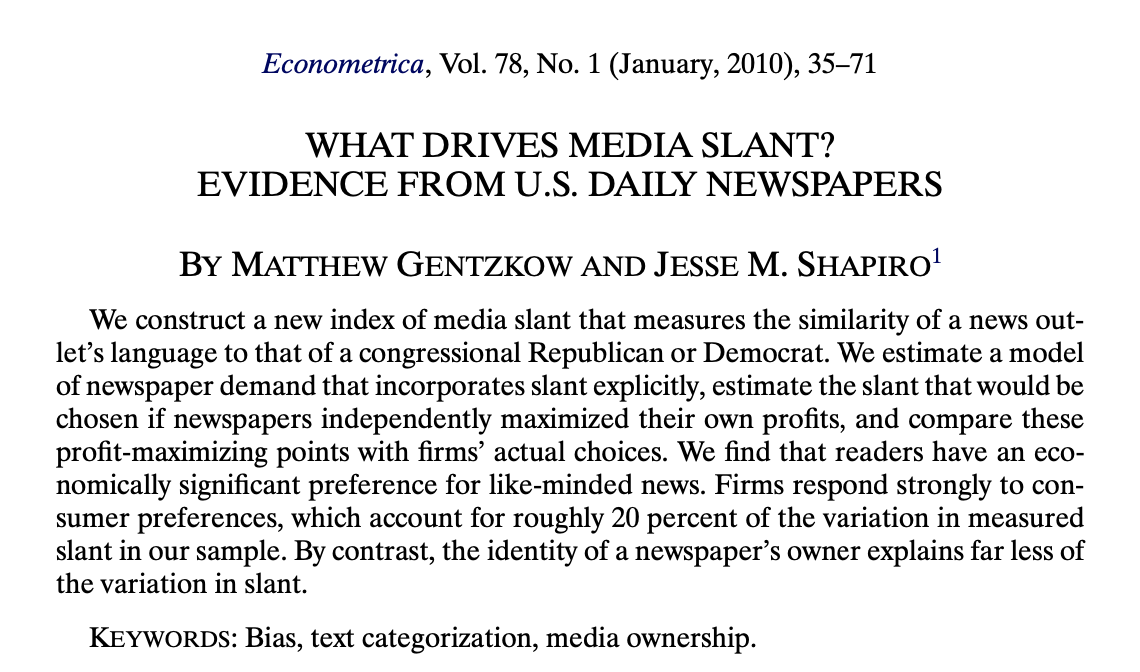
\includegraphics[scale=0.5]{figures/gentzgow_shapiro}
              
 \end{figure}

\end{frame}
%----------------------------------------------------------------------%
\begin{frame}[fragile]
\frametitle{Text as Data: Motivation}
\framesubtitle{Gentzkow and Shapiro: What drives media slant?  Evidence from U.S. daily newspapers ({\it Econometrica}, 2010)}

\begin{itemize}
\item Construir un modelo económico para la demanda de los periódicos que incorpore el partidismo político (\rd republicano \bk vs \bl demócrata \bk)


 
\begin{itemize}
\item ¿Cuál sería la ``inclinación'' independiente de maximización de beneficios?
\item Compare esto con el sesgo estimado a partir del texto del periódico.
\end{itemize}
\end{itemize}

\begin{center}
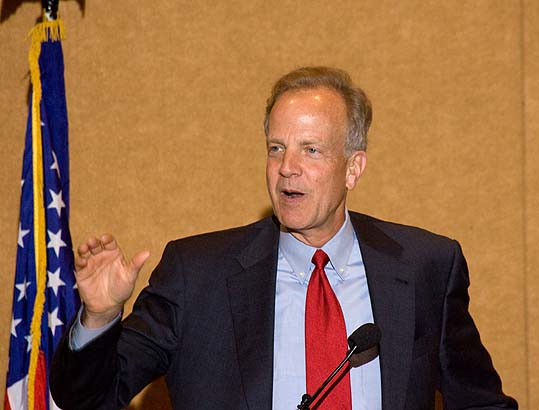
\includegraphics[width=1.7in]{figures/moran}
~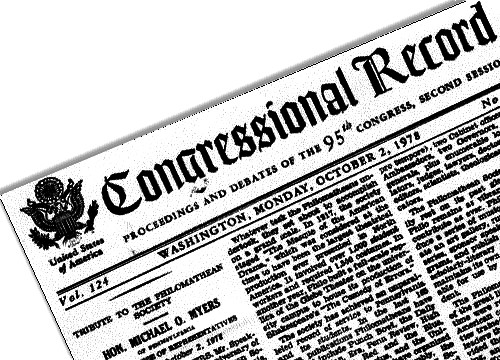
\includegraphics[width=1.75in]{figures/record}
\end{center}


 \end{frame}
%----------------------------------------------------------------------%
\begin{frame}[fragile]
\frametitle{Text as Data: Motivation}

\begin{itemize} 
\item Jerry Moran, R-KS, dice ``death tax'' a menudo y su distrito  votó 73\% por George W. Bush en 2004.
\end{itemize}

\begin{center}
$\bm{X_\text{text}} = f( \text{ideology}) \approx g(Y_{Bush})$

\vskip .25cm
$\bm{\Rightarrow}$ ``death tax'' es republicano

\vskip .25cm
$\Rightarrow $ \theme el Wall Street Journal se inclina a la derecha.

\medskip
\begin{itemize} 
\item William Jefferson, D-LA, dice ``estate tax'' a menudo y su distrito votó 24\% por George W. Bush en 2004.
\end{itemize}
\end{center}


\end{frame}

%----------------------------------------------------------------------%
\begin{frame}[fragile]
\frametitle{Text as Data: The Big Picture}

\begin{itemize}


\item {\bf \theme Text is a vast source of data for business }
\medskip
\item It comes connected to interesting ``author'' variables 
\medskip
  \begin{itemize}
  \item What you buy, what you watch, your reviews
  \medskip
  \item Group membership, who you represent, who you email
  \medskip
  \item Market behavior, macro trends, the weather
  \end{itemize}

 
\item Opinion, subjectivity, etc.
\medskip
\item  Sentiment is {\it very} loosely defined:  Observables linked to the variables motivating language choice
\end{itemize}

\end{frame}
%----------------------------------------------------------------------%
\begin{frame}[fragile]
\frametitle{Text as Data: The Big Picture}

\begin{itemize}

\item {\bf \theme Text is also super high dimensional }

\medskip
\item And it gets higher dimensional as you observe more speech.


\medskip
\item Analysis of  phrase counts is the state of the art (hard to beat).

\end{itemize}

\end{frame}

%----------------------------------------------------------------------%
\section{Aspectos Operativos}
%----------------------------------------------------------------------%
%----------------------------------------------------------------------%
\begin{frame}[fragile]
\frametitle{}


\centering
{\huge \textcolor{andesred}{Aspectos Operativos}}


\end{frame}


%----------------------------------------------------------------------%
\subsection{Tokenization}
%----------------------------------------------------------------------%
\begin{frame}[fragile]
\frametitle{Information Retrieval and Tokenization}

\begin{itemize}


\item A passage in `{\it As You Like It}' from Shakepeare:

\medskip

~~~ {\sg All the world's a stage,\\
~~~ and all the men and women merely players:\\
~~~ they have their exits and their entrances;\\
~~~ and one man in his time plays many parts...}


\medskip
\item What the econometrian sees:

\medskip
\vspace{-.4cm}{\sg
\begin{verbatim}
   world stage men women play exit entrance time 
       1     1   2     1    2    1        1    1 
\end{verbatim}}

\medskip
\item This is the {\nv Bag-of-Words} representation of text.
\end{itemize}
\end{frame}

%----------------------------------------------------------------------%
\begin{frame}[fragile]
\frametitle{Possible tokenization steps} 

\begin{itemize}


\item Remove words that are super rare {\gr (in say $<\frac{1}{2}$\%, or $<15\%$ of docs; this is application specific)}.
 For example, if {\nv Argentine} occurs only once, it's useless for comparing documents.


\item Stemming:  `{\nv tax}' $\leftarrow$   taxing,  taxes, taxation, taxable, ... 

{\gr A stemmer cuts words to their root with a mix of rules and estimation.`Porter' is standard for English. }



\item  Remove a list of {\nv stop words} containing  irrelevant tokens.

{\gr ~~~~~If, and, but, who, what, the, they, their, a, or, ...}

{\nv Be careful: one person's stopword is another's key term.}


\item Convert to lowercase, drop numbers, punctuation, etc ...\\
{\gr Always application specific: e.g., don't drop {\tt :-)} from tweets.}
\end{itemize}


\end{frame}


%----------------------------------------------------------------------%
\begin{frame}[fragile]
\frametitle{The $n$-gram language model}

\begin{itemize}

\item An $n$-gram language model is one that describes a dialect through transition probabilities on $n$ consecutive words.

\medskip

\item An {\theme $n$-gram tokenization} counts length-$n$ sequences of words.\\
{\sg A unigram is a word, bigrams are transitions between words.}\\
{\gr e.g., {\tt world.stage}, {\tt stage.men}, {\tt men.women}, {\tt women.play}, ...}

\medskip

\item This can give you rich language data, but be careful: $n$-gram token vocabularies are very high dimensional ($p^n$)
\medskip
\item  More generally, you may have domain specific `clauses' that you wish to tokenize.
\medskip
\item  There is always a trade-off between complexity and generality. 
\medskip
\item {\theme Often best to just count words.}

\end{itemize}


\end{frame}
%----------------------------------------------------------------------%
\begin{frame}[fragile]
\frametitle{Text as Data: Wordle} 

\begin{itemize}
  \item {\theme Often best to just count words.}
  \medskip
  \item For example, occurrences by party for some partisan terms

  \vskip .25cm
  {\footnotesize
  \begin{tabular}{|c|c|c|c|c|c|c}
  Congress & State & Party & America & Death Tax & Estate Tax & $\cdots$
  \\ \hline
  \multirow{2}{*}{63} & \multirow{2}{*}{\sf NM} & {\sf dem}  & 108 &
    30 & 140 & \\ &
  & {\sf gop}  & 100 &
    220 & 12  &
  \end{tabular}}

\begin{figure}[H] \centering
            \captionsetup{justification=centering}
              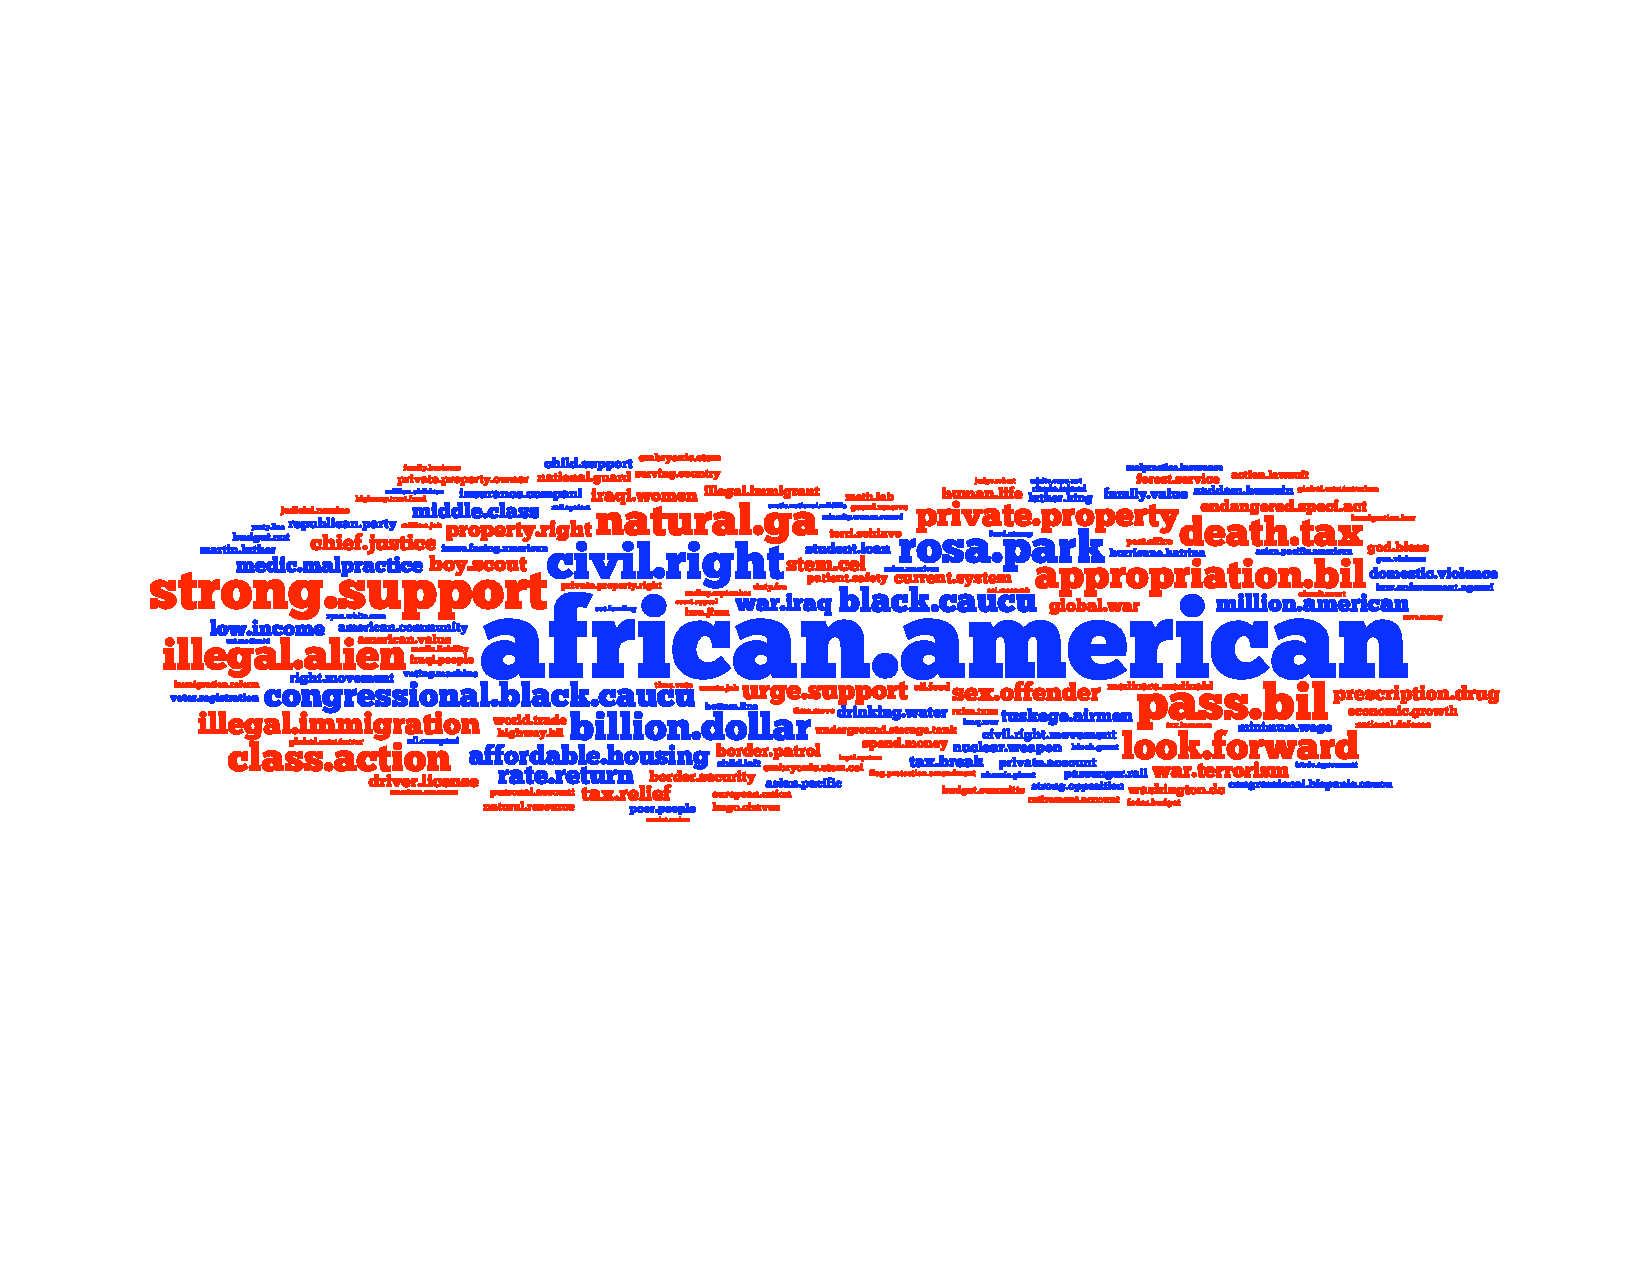
\includegraphics[width=4.5in]{figures/slantWrdl}
              
 \end{figure}

\end{itemize}



\end{frame}
%----------------------------------------------------------------------%
\begin{frame}
\frametitle{Text Regression}

\begin{itemize}
\item Once you have text in a numeric format, we can use all the tools we learned so far

\medskip
\begin{align}
y= f(word\,counts) + u
\end{align}
 
\item where you can use lasso, PCA, etc. to do dimentionality reduction

\end{itemize}
\end{frame}
%----------------------------------------------------------------------%
\begin{frame}
\frametitle{Text Regression}

\begin{center}
{\bf Slant measure for speakers in the 109th Congress}
\vskip -.5cm
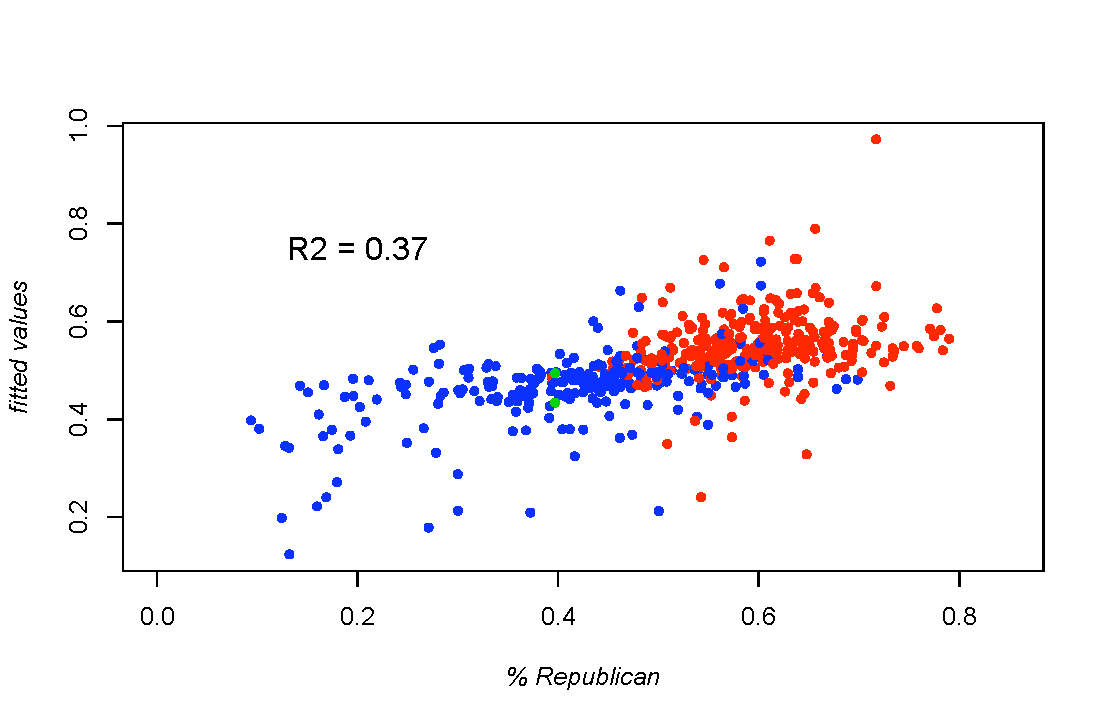
\includegraphics[width=4in]{figures/slant}\\
\end{center}

\vskip -.5cm
Democrats get low $z_\text{slant}$ and Republicans get high
$z_\text{slant}$.\\
\gr Do this for newspaper text and you'll get a similar picture

\end{frame}
%----------------------------------------------------------------------%
\begin{frame}
\frametitle{Text Regression}


\begin{itemize}
\item Another example: Classify emails into spam

\begin{figure}[H] \centering
            \captionsetup{justification=centering}
              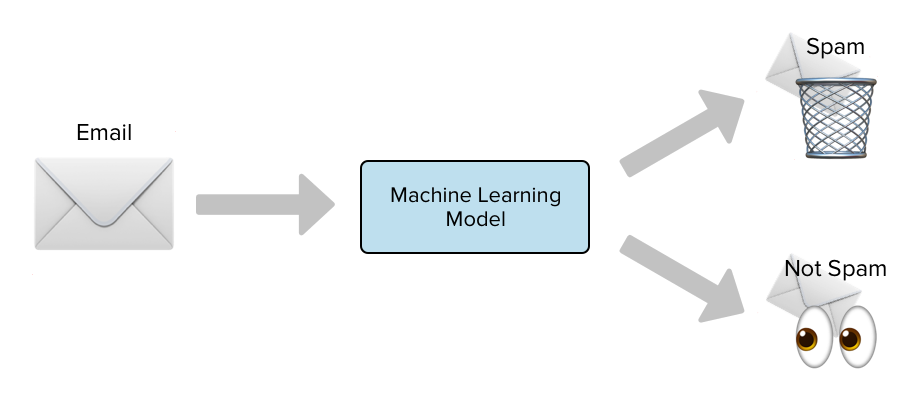
\includegraphics[width=4in]{figures/spam}
              
 \end{figure}

\medskip
\begin{align}
\mr{logit}\left[{\tt spam} \right] = \alpha + f \beta
\end{align}
\item where $f_i=\frac{x_i}{\sum_j x_{ij}}$ are the normalized text counts
\end{itemize}
\end{frame}
%----------------------------------------------------------------------%
\section{Modelos de Tópicos}
%----------------------------------------------------------------------%
%----------------------------------------------------------------------%
\begin{frame}[fragile]
\frametitle{}


\centering
{\huge \textcolor{andesred}{Modelos de Tópicos}}


\end{frame}
%----------------------------------------------------------------------%
\section{Modelos de Tópicos}
%----------------------------------------------------------------------%
\begin{frame}
\frametitle{Topic Models}

\begin{itemize}
\item Text is super high dimensional
\medskip
\item there is often abundant {\it unlabeled} text
\medskip
\item Some times unsupervized factor model is a popular and useful strategy with text data
\medskip
\item You can first fit a factor model to a giant corpus and use these factors for supervised learning on a subset of labeled documents.
\medskip
\item The unsupervised dimension reduction facilitates the supervised learning
\end{itemize}
\end{frame}
%----------------------------------------------------------------------%
\begin{frame}
\frametitle{Topic Models: Example}

\begin{itemize}


\item We have 6166 reviews, with an average length of 90 words per review, \url{we8there.com}. 
\medskip
\item A useful feature of these reviews is that they contain both text and a multidimensional rating on overall experience, atmosphere, food, service, and value. 
\medskip
\item For example, one user submitted a glowing review for Waffle House \#1258 in Bossier City, Louisiana: 
\medskip
{\tt \it 
I normally would not revue a Waffle House but this one deserves it. The workers, Amanda, Amy, Cherry, James and J.D. were the most pleasant crew I have seen. While it was only lunch, B.L.T. and chili, it was great. The best thing was the 50’ s rock and roll music, not to loud not to soft. This is a rare exception to what you all think a Waffle House is. Keep up the good work. \\
Overall: 5, Atmosphere: 5, Food: 5, Service: 5, Value: 5. 
}
\end{itemize}
\end{frame}
%----------------------------------------------------------------------%
\begin{frame}[fragile]
\frametitle{Topic Models: Example}
\begin{itemize}


\item Puedo resumir estos textos a algunos simples temas?
\medskip
\item Puedo usar PCA
\medskip
\item Tambien podemos usar LDA (más apropiado)
\end{itemize}

\end{frame}
%-------------------------------------%
\begin{frame}[fragile]
\frametitle{Principal Component Regression}


\begin{itemize}




\item The concept is very simple: instead of regressing onto $X$, use a lower dimension set of principal components $F$ as covariates.

\medskip
\item This works well for a few reasons:
\begin{itemize}
\item PCA reduces dimension, which is always good.
\item Higher variance covariates are good in regression, and we choose
  the top PCs to have highest variance.
\item The PCs are independent: no multicollinearity.
\end{itemize}


\item The 2-stage algorithm is straightforward. For example,

{\nv 
\begin{semiverbatim}\vspace{.25cm}\small
         mypca = prcomp(X, scale=TRUE)
         z = predict(mypca)[,1:K]
         reg = glm(y~., data=as.data.frame(z))
\end{semiverbatim}
}

\end{itemize}


\end{frame}

%----------------------------------------------------------------------%
\subsection{Latent Dirichlet Allocation}
%----------------------------------------------------------------------%
\begin{frame}
\frametitle{Latent Dirichlet Allocation}

\begin{itemize}


\item The approach of using PCA to factorize text was common before the 2000s. 
\medskip
\item Versions of this algorithm were referred to under the label latent semantic analysis. 
\medskip
\item However, this changed with the introduction of topic modeling, also known as Latent Dirichlet Allocation (LDA), by Blei et al. in 2003. 
\medskip
\item These authors pointed out that the squared error loss (i.e., Gaussian model) implied by PCA is inappropriate for analysis of sparse word-count data. 
\medskip

\end{itemize}

\end{frame}
%----------------------------------------------------------------------%
\begin{frame}
\frametitle{Latent Dirichlet Allocation}

\begin{figure}[H] \centering
            \captionsetup{justification=centering}
              
\includegraphics[width=4in]{figures/hansen1.png}
              
 \end{figure}

 \end{frame}
%----------------------------------------------------------------------%
\begin{frame}
\frametitle{Latent Dirichlet Allocation}

\begin{figure}[H] \centering
            \captionsetup{justification=centering}
              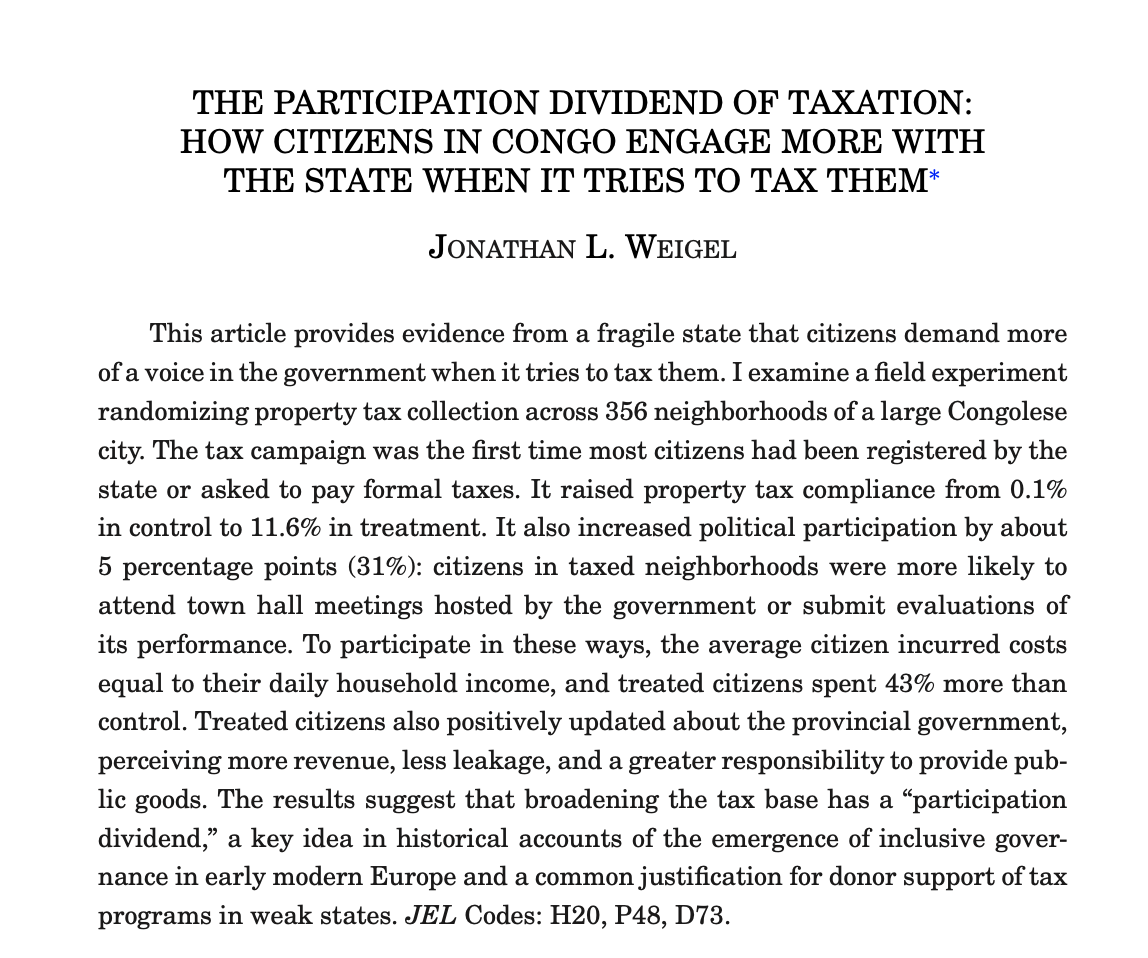
\includegraphics[scale=0.4]{figures/weigel1.png}
              
 \end{figure}

 \end{frame}
%----------------------------------------------------------------------%
\begin{frame}
\frametitle{Latent Dirichlet Allocation}

\begin{figure}[H] \centering
            \captionsetup{justification=centering}
              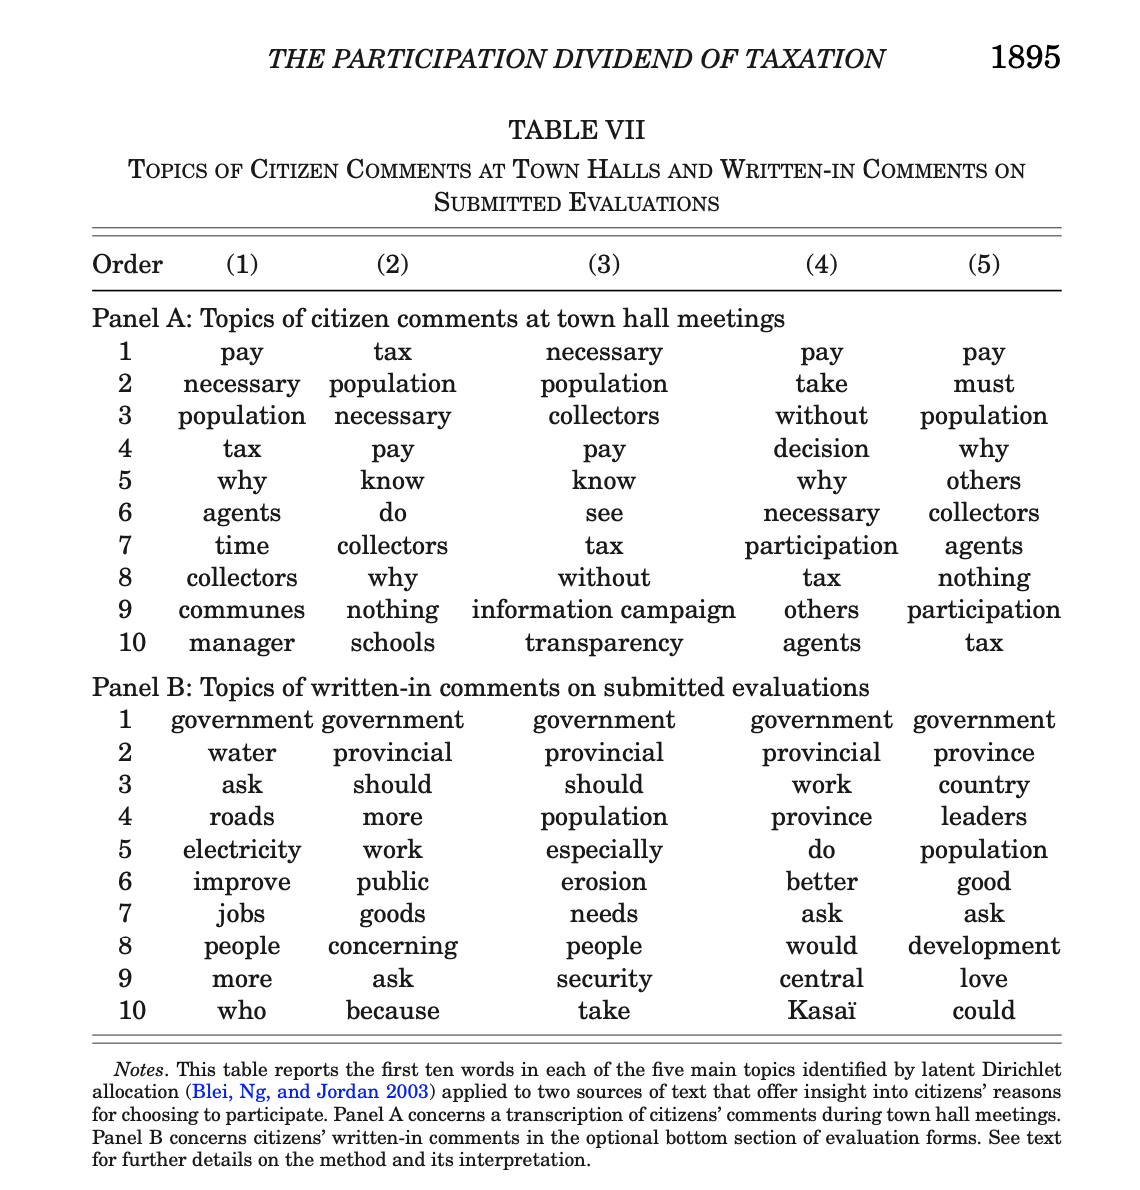
\includegraphics[scale=0.4]{figures/weigel2.png}
              
 \end{figure}


\end{frame}
%----------------------------------------------------------------------%
\begin{frame}
\frametitle{Latent Dirichlet Allocation}

\begin{itemize}
\item Blei et al. proposed you take the bag-of-words representation seriously and model token counts as realizations from a multinomial distribution. 

\medskip
\item Topic models are built on a simple document generation process: 
\medskip
\begin{itemize}

\item  For each word, pick a “topic” k. This topic is defined through a probability vector over words, say, $\theta_k$ with probability $\theta_{kj}$ for each word j. 
\medskip
\item Then draw the word according to the probabilities encoded in $\theta_k$ . 
\medskip
\end{itemize}
\item After doing this over and over for each word in the document, you have proportion $\omega_{i1}$ from topic 1, $\omega_{i2}$ from topic 2, and so on. 

\end{itemize}
\end{frame}
%----------------------------------------------------------------------%
\begin{frame}
\frametitle{Latent Dirichlet Allocation}

\begin{itemize}


\item This basic generation process implies that the full vector of word counts, $x_i$, has a multinomial  distribution: 
\medskip
\begin{align}
x_i \sim MN(\omega_{i1}\theta_1+\dots+\omega_{iK}\theta_K,m_i)
\end{align}
\medskip
\item where $m_i=\sum_j x_{ij}$ is the total document length and, for example, 
\medskip
\item the probability of word j in document i will be $\sum_k \omega_{ik}\theta_{kj}$

\end{itemize}


\end{frame}
%----------------------------------------------------------------------%
\begin{frame}
\frametitle{Latent Dirichlet Allocation vs PCA}

\begin{itemize}
\item Recall our PC model:
\medskip
\begin{align}
E(x_i) = \delta_{i1} F_1 + \dots + \delta_{iK} F_K
\end{align}

\medskip
\item The analogous topic model representation, implied by the above equation, is
\medskip
\begin{align}
E(\frac{x_i}{m_i}) = \omega_{i1} \theta_1 + \dots + \omega_{iK} \theta_K
\end{align}

 

\item such that topic score $\omega_{ik}$ is like PC score $\delta_{ik}$ and 
\item $\theta_k$ topic probabilities are like rotations $F_k$. 
\item The distinction is that the multinomial in implies a different loss function ( from a multinomial) rather than the sums of squared errors that PCA minimizes. 
\item Note that we condition on document length here so that topics are driven by relative rather than absolute term usage. 
\end{itemize}

\end{frame}

%----------------------------------------------------------------------%
\section{Word Embeddings}
%----------------------------------------------------------------------%
%----------------------------------------------------------------------%
\begin{frame}[fragile]
\frametitle{}


\centering
{\huge \textcolor{andesred}{Word Embeddings}}


\end{frame}


%----------------------------------------------------------------------%
\section{Word Embedding }
%----------------------------------------------------------------------%
\begin{frame}
\frametitle{Word Embedding }

\begin{itemize}
\item This is a new method  that have come out of work in deep learning. 
\medskip
\item Word embedding was originally motivated as a technique for dimension reduction on the inputs to a deep neural network. 
\medskip
\medskip
\item However, word embedding turns out to be valuable in its own right: it imposes a spatial structure on words, making it possible for those studying language to reason about distances between meanings and consider the algebra behind combinations of words in documents. 


\end{itemize}




\end{frame}
%----------------------------------------------------------------------%
\begin{frame}
\frametitle{Word Embedding }

\begin{itemize}
  \item In the original deep learning context, embedding layers replace each word with a vector value, such that, for example, hotdog becomes the location [1,–5, 0.25] in a three-dimensional embedding space% (this is just for illustration; embedding spaces are typically of more than 100 dimensions). 
  \item Compare this to the standard bag-of-words representation, where hotdog would be represented as a binary vector that is as long as there are words in the vocabulary, say, p. 
  \medskip
  \item This binary vector will have p–1 zeros and a one in the hotdog dimension. 
  \medskip
  \item The word embedding has translated the language representation from a large binary space to a smaller real-valued (and much richer) space. 
\end{itemize}


\end{frame}
%----------------------------------------------------------------------%
\begin{frame}
\frametitle{Word Embedding }

\begin{itemize}
\item There are a variety of different embedding algorithms—as many as there are different architectures for deep neural networks. 
\medskip
\item The most common and general embeddings are built around word co-occurrence matrices. 
\medskip
\item This includes the popular \texttt{Glove} and \texttt{Word2Vec} frameworks. 
\medskip
\item What is co-occurrence?
  \begin{itemize}
  \item  Two words co-occur if they appear within the same sentence and within b words of each other. Where b is the “window size”
  \item  For a vocabulary size p, this leads to a sparse p × p co-occurrence matrix where each [i, j] entry is the number of times that words i and j co-occur. Call this matrix C. 
  \item A word embedding algorithm seeks to approximate C as the product of two lower-dimensional matrices
  \end{itemize}
\end{itemize}
 
\end{frame}
%----------------------------------------------------------------------%
\begin{frame}
\frametitle{Word Embedding }

\begin{itemize}
  \item A word embedding algorithm seeks to approximate C as the product of two lower-dimensional matrices
  \begin{align}
  C\approx UV'
  \end{align}

  \item Here, U and V are each $p \times K$ dimensional dense and real valued matrices. 
  \item K is the dimension of the embedding space; hence, $K < < p$ and both U and V are very tall and thin matrices. 
  \item Each row of U and of V, $u_j$ and $v_j$ is then a K-dimensional embedding of the jth word. 
  \item The implication is  that these embeddings summarize the meaning of words as their inner product defines how much you expect them to co-occur. 
  \\
  {\footnotesize Recall that the inner product is a standard measure of distance in linear algebra (e.g. $e'e$)}

  
\end{itemize}

 
\end{frame}
%----------------------------------------------------------------------%
\begin{frame}
\frametitle{Word Embedding }

\begin{itemize}
\item One way to find U and V is to solve $C\approx UV'$ through the singular value decomposition (SVD).
\item SVD is a factorization of a real or complex matrix, that serves for example, to find the eigenvalues and eigenvectors of square symmetric matrices (and hence in calculating principal components). 
\item In practice, most of the software embedding solutions use alternatives to SVD that are designed to deal with the high amount of sparsity in C (since most words never co-occur in limited windows for standard corpora). 

\item Under many algorithms, especially when co-occurrence is symmetric, U and V will be mirror images of each other. 
\item Thus, it is standard to take one of these vectors $u_j$ as the single embedding location for word j.
\end{itemize}


\end{frame}
%----------------------------------------------------------------------%
\begin{frame}
\frametitle{Word Embedding }

\begin{itemize}


 \item These locations were originally viewed as an intermediate output—as a processing step for inputs to a deep neural network.
\item However, social scientists and linguists have discovered that the space of word locations contains rich information about the language of the documents used to train the embedding. 


\item Word embeddings preserve semantic relationships.
  \begin{itemize}
    \item Words with similar meaning have similar representations.
    \medskip
    \item Dimensions induced by word differences can be used to identify cultural concepts 
  \end{itemize}
  \item For example, the vector difference \texttt{man - woman} isolates a gender dimension in the space.
  \medskip
  \item  The dimensions are useful because they produce quantitative measures of similarity between the associated concepts and specific words in the corpus. 
  \end{itemize}


\end{frame}

%----------------------------------------------------------------------%
\begin{frame}
\frametitle{Word Embedding }

\begin{itemize}
  \item In this case, we can understand the gender connotation of a given word by taking the cosine of the angle between the vector representation of the word and the differenced vector representing the gender dimension 
  \medskip 
\item This is because the cosine of the angle, can be interpreted as a similarity measure.
\medskip
\item The similarity ranges from -1 meaning exactly opposite, to 1 meaning exactly the same, with 0 indicating orthogonality or decorrelation, while in-between values indicate intermediate similarity or dissimilarity. 
\end{itemize}

  \begin{figure}[H] \centering
            \captionsetup{justification=centering}
              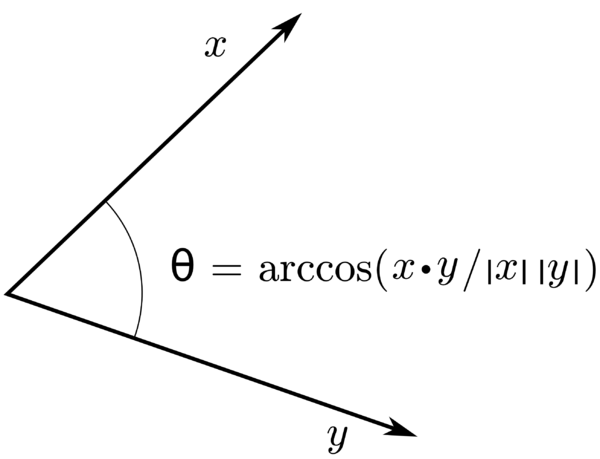
\includegraphics[scale=0.14]{figures/Inner_product_angle.png}
              
 \end{figure}


\end{frame}
%----------------------------------------------------------------------%
\begin{frame}
\frametitle{Word Embedding }
\begin{itemize}



\item Words with male connotations – e.g. male first names – are going to be positively correlated with \texttt{man - woman}.
\medskip
\item Female words, in turn, will be negatively correlated with the dimension.
\medskip
\item This framework provides an intuitive approach to measuring stereotypical associations in a given corpus. 
\medskip
\item Bolukbasi et al (2016) is a nice example
\end{itemize}

 \end{frame}
%----------------------------------------------------------------------%
\begin{frame}
\frametitle{Word Embedding: Example 1 }


  \begin{figure}[H] \centering
            \captionsetup{justification=centering}
              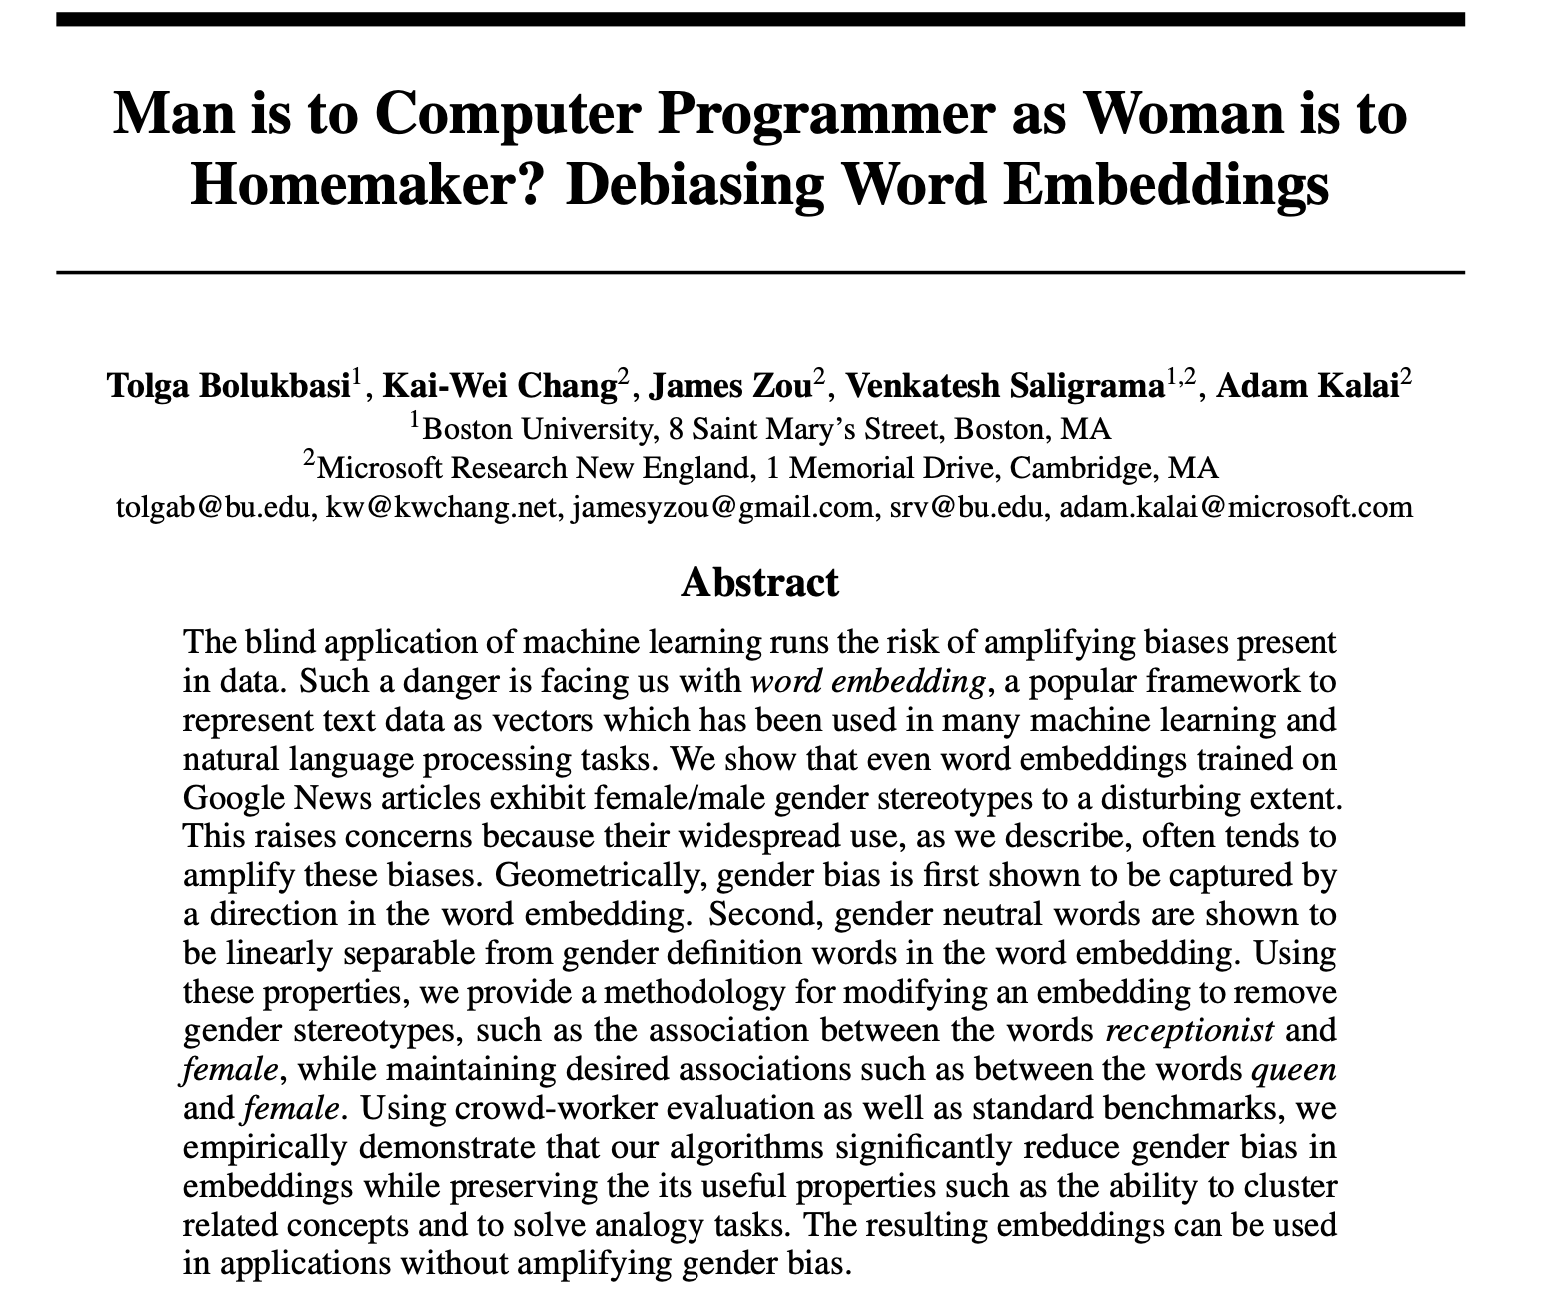
\includegraphics[scale=0.3]{figures/bolukbasi}
              
 \end{figure}

 \end{frame}
%----------------------------------------------------------------------%
\begin{frame}
\frametitle{Word Embedding: Example 1 }

\begin{itemize}


\item They trained a standard word2vec embedding algorithm on the Google News corpora of news articles. 
\item Then look at the differences between established gender words (for example, the vector for man minus the vector for woman, or father minus mother) to establish an axis in the embedding space that spans from masculinity to femininity. 
\item They then calculate the location along this axis for a large number of terms that should be gender-neutral. 
\item  The embedding space has learned—from how the words are used in news articles—that these professions are stereotypically viewed as female and male occupations.
\end{itemize}

\end{frame}
%----------------------------------------------------------------------%
\begin{frame}
\frametitle{Word Embedding: Example 1 }


  \begin{figure}[H] \centering
            \captionsetup{justification=centering}
              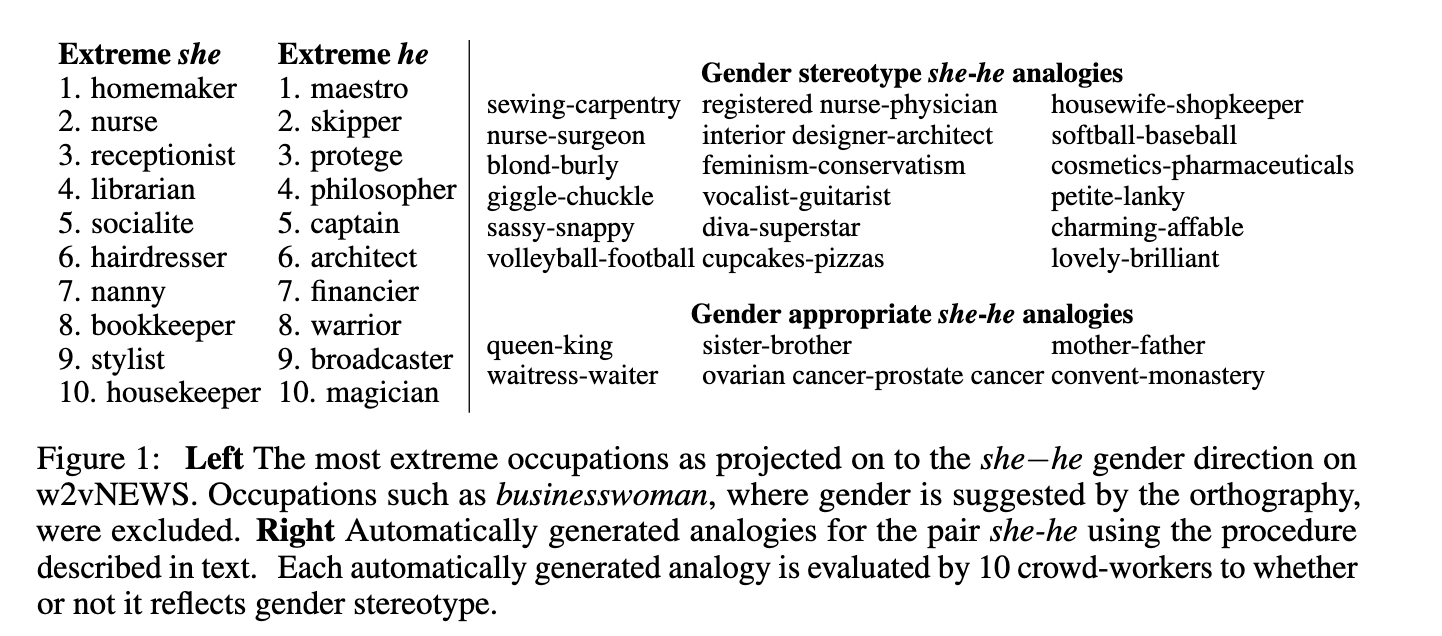
\includegraphics[scale=0.5]{figures/bolukbasi_2}
              
 \end{figure}

\end{frame}

%----------------------------------------------------------------------%
\begin{frame}
\frametitle{Word Embedding: Example 2 }


  \begin{figure}[H] \centering
            \captionsetup{justification=centering}
              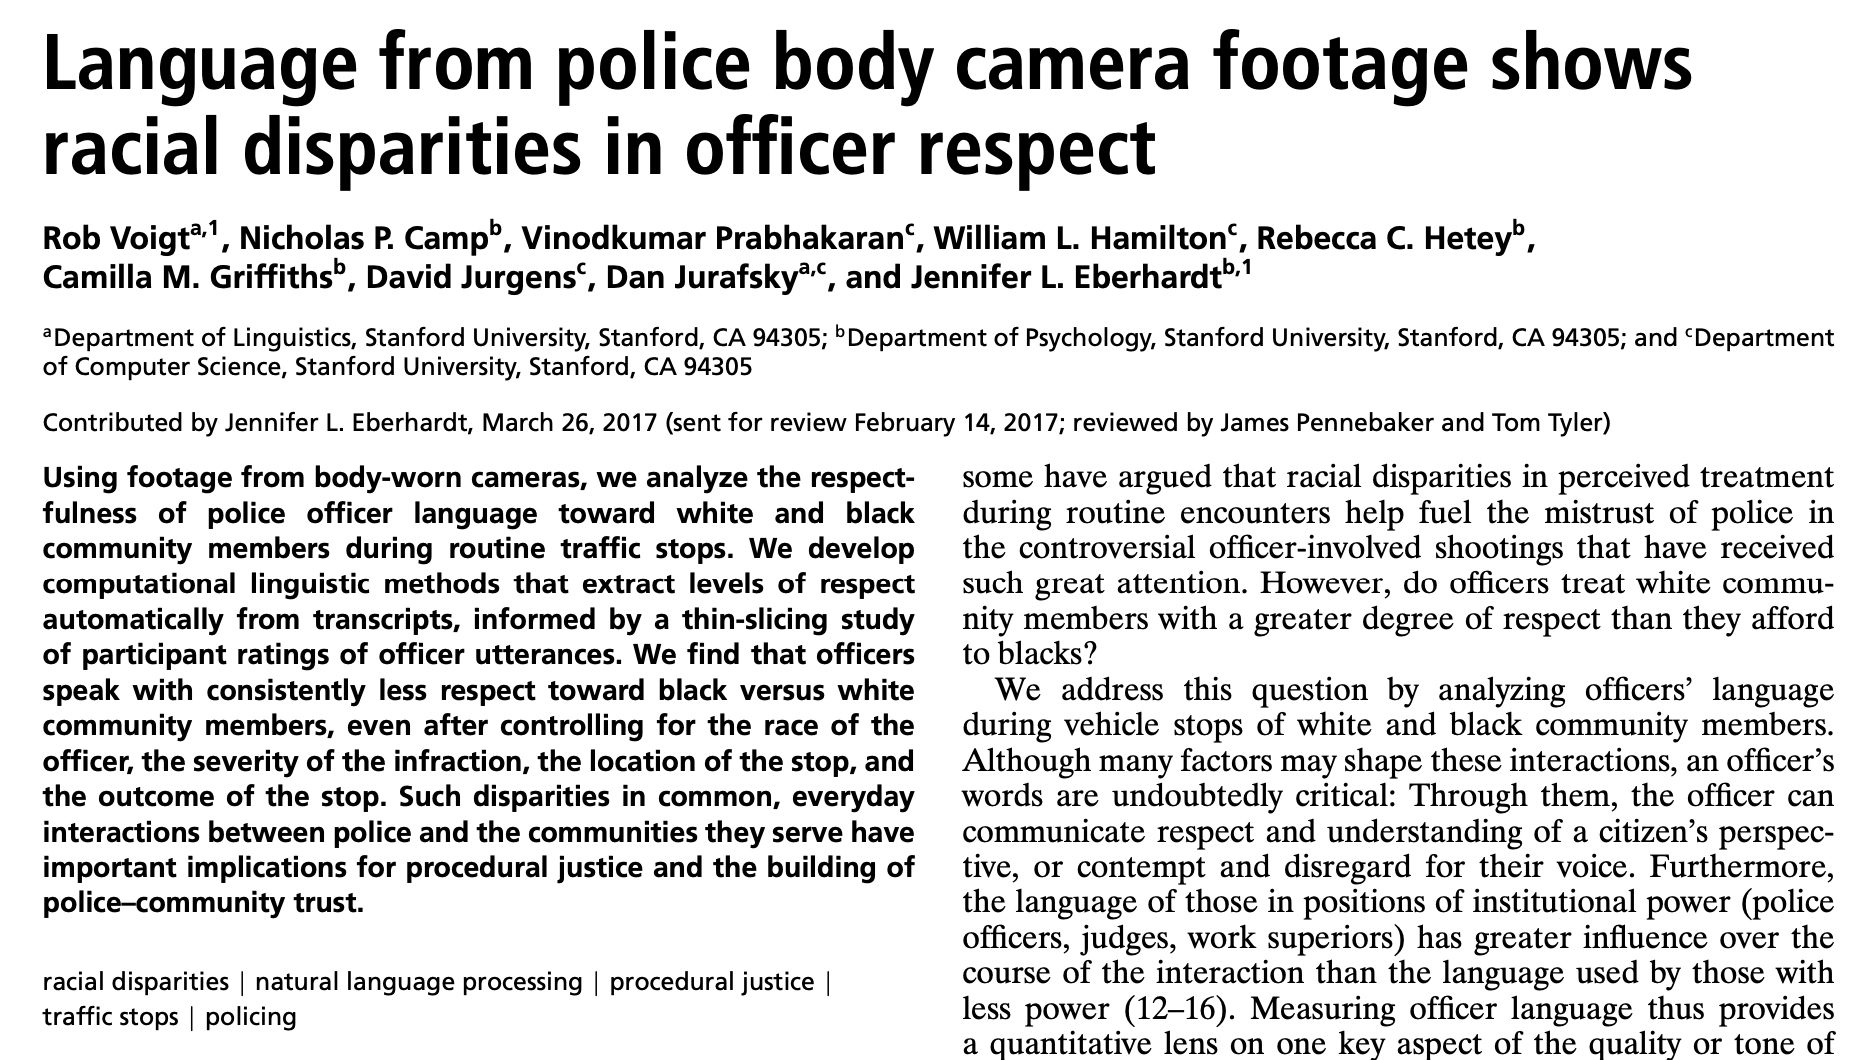
\includegraphics[scale=0.4]{figures/body_camera}
              
 \end{figure}

\end{frame}
%----------------------------------------------------------------------%
\begin{frame}
\frametitle{Word Embedding: Example 3 }


  \begin{figure}[H] \centering
            \captionsetup{justification=centering}
              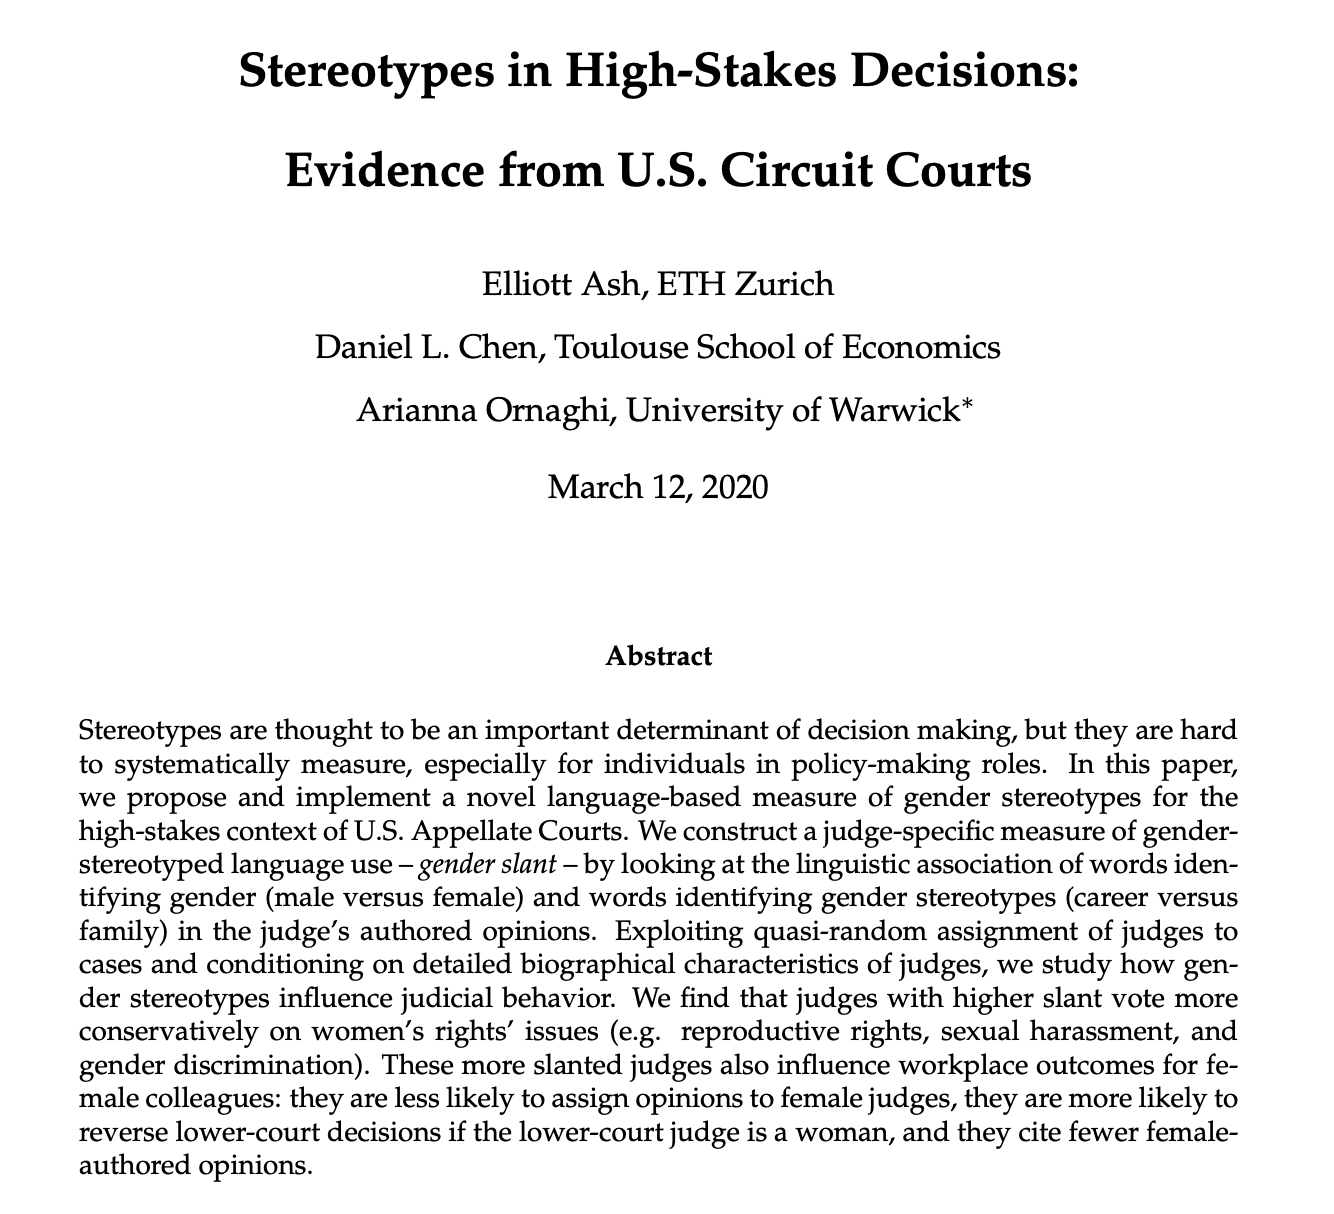
\includegraphics[scale=0.35]{figures/high_stakes_decisions}
              
 \end{figure}

\end{frame}


%----------------------------------------------------------------------%
\section{Break}
\begin{frame}
\frametitle{}

\begin{centering}
\huge
\textcolor{andesred}{Volvemos en 15 mins con \texttt{R} }

\end{centering}

\end{frame}
%----------------------------------------------------------------------%
\section{\texttt{R para ML}}
%----------------------------------------------------------------------%
\begin{frame}
\frametitle{R para ML}

\begin{figure}[H] \centering
  \centering
  
\includegraphics[scale=0.35]{../Lecture04/figures/baticomputer_meme.jpg}
  \\
  \tiny photo from \url{https://www.dailydot.com/parsec/batman-1966-labels-tumblr-twitter-vine/}
\end{figure}

\end{frame}




%----------------------------------------------------------------------%
\begin{frame}[fragile]
\frametitle{Text as Data: What is slant?}

\begin{itemize}
\item { Text:}  phrase-counts by speaker in 109$^{th}$ US Congress
(05-06)
\medskip
\item  { Sentiment:} two-party constituent vote-share for Bush in 2004.
\medskip

\item  Use covariance between  phrase frequencies ($f_{ij}$) and `Bush' sentiment ($y_i$)  to build an index of partisanship for text. 
\begin{center}\large
$z^{slant}_i= \sum_j \mr{cov}(f_j, y) f_{ij}$
\end{center}
\medskip
 \item For example, if phrase $j$ forms  a high proportion of what you say, and usage of phrase
 \medskip
\item $j$ is correlated with Bush vote-share, then this contributes a positive amount to your slant score.
\medskip
\vskip .2cm
\item  This is a type of {\it marginal regression}.
\end{itemize}
\end{frame}


%----------------------------------------------------------------------%
%----------------------------------------------------------------------%
\end{document}
%----------------------------------------------------------------------%
%----------------------------------------------------------------------%